\documentclass[a4paper,10pt]{article}
\usepackage[utf8]{inputenc}
\usepackage{amsmath, amsfonts, graphicx}
%opening
\title{Optical geometry of cameras}
%\author{Vahagn Eghikian}

\begin{document}

\maketitle

%\begin{abstract}

%\end{abstract}

\section{Introduction}
Here should be the introduction.
\section{Camera}

Any camera is comprised of a lens, an aperture disk and a sensor. 

\subsection{ The Pinhole Camera}

Let us assume that we have a light emitting point in 3D space and a 2D sensor. If we place the point in front of the sensor the emitted rays  will fully cover the  sensor's surface and we will not receive any valuable information other than the acknowledgment of a bright point next to our sensor -  Figure \ref{fig:point_and_sensor}.

\begin{figure}[h]
\centering
 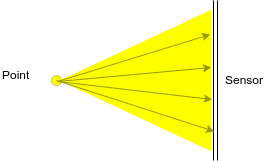
\includegraphics[width=0.6\textwidth]{../../images/point.png}
 \caption{The light from the point covers the whole sensor}
 \label{fig:point_and_sensor}
\end{figure}

To get a more detailed picture, let us place a black screen with a tiny hole between the sensor and the point. If the hole is small enough only the rays which connect the point to the hole will pass the screen and we will project our point in space on a single point on our sensor.  Figure \ref{fig:pinhole} illustrates the described process. 
\begin{figure}[h]
\centering
 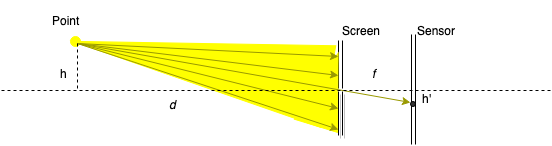
\includegraphics[width=0.9\textwidth]{../../images/pinhole_point.png}
 \caption{Only a single point on the sensor is illuminated by the light emitted from the point}
 \label{fig:pinhole}
\end{figure}

The axis orthogonal to the screen (and the sensor) and passing through the hole is called {\it principal axis}. The distance from the screen to the sensor is called {\it focal length}. 

It is clear from Figure \ref{fig:pinhole} that objects in general will appear upside down on the sensor. 

Using similarity relations between triangles it is easy to derive the following formula:

\begin{equation}                                                                                                                                                                         
h' = h\frac{f}{d}
\label{pinhole_ratio}
\end{equation}

Let us rewrite this formula in the coordinate language. Let us introduce  the 3D world coordinate system  with axes $(X,Y,Z)$ and 2D image coordinate system with axes $(x,y)$ as shown in Figure \ref{fig:pinhole_coordinates}.

\begin{figure}[h]
\centering
 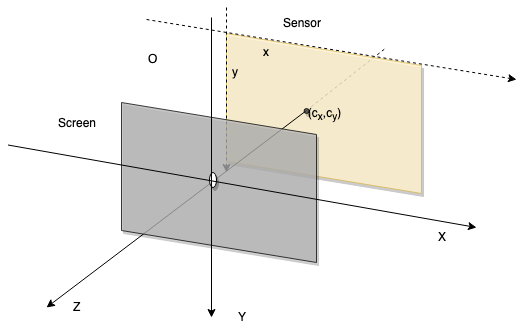
\includegraphics[width=0.9\textwidth]{../../images/pinhole_coords.png}
 \caption{World and image coordinate systems}
 \label{fig:pinhole_coordinates}
\end{figure}

If we first place the origin of the image coordinate system in the point where the principal axis intersects the sensor plane the \eqref{pinhole_ratio} leads to:
$$
\left\{\begin{array}{c}
x = f \frac{X}{Z} \\
y = f \frac{Y}{Z} 
\end{array}\right.
$$

In the digital world, however, the origin of the coordinate system on the image is placed in the top left corner of the image(sensor) so all points $(0,0,Z)$ are projected to the principal point $(c_x, c_y)$.  To include this, we rewrite the formulae as follows:  

\begin{equation}
\left\{\begin{array}{c}
x = f \frac{X}{Z} + c_x\\ 
y = f \frac{Y}{Z} + c_y
\end{array}\right.\label{projinhmg}
\end{equation}
This is the so-called {\it projection formula} for pinhole camera. In the upcoming posts we will linearize it  and represent in a matrix form. 

In the end of this section, let us notice that in order to project a point on a point the described method requires the hole on the screen to be as small as possible, ideally - a point.  In the real world, however, it is impossible to make an infinitely small hole. When it has finite size the image of the point turns into a disk - the {\it circle of confusion  } Fig 3.
\begin{figure}[h]
\centering
 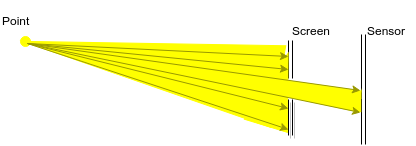
\includegraphics[width=0.6\textwidth]{../../images/confusion_circle.png}
 \caption{}
\end{figure}

Obviously, the wider the hole the the bigger the  circle of confusion. Also, the closer the point to the screen, the wider the confusion circle. 

{\bf\tiny An interesting fact: the stars are so far from us, that the rays coming from them are almost parallel and, therefore, the diameter of the confusion circle is equal to the diameter of the hole on the screen.}

However, due to a number of reasons we cannot make the hole very small.

First of all a smaller hole means less light reaching the sensor and, as a result,  dimmer pictures. On the other hand, if, for example,  we use a digital sensor, and  make the hole so small that in the distance range interesting for us the confusion circle is not bigger than a pixel on the sensor; no matter how small we make the hole, our picture will not get any sharper, it will rather get dimmer and dimmer until vanishes in the noise of the device.

The second and, probably not very actual, reason is that even if we could amplify the light coming from the objects or make the sensor's pixels infinitely sensitive there is another effect which emerges when the radius of the hole becomes comparable to the wavelength of the optical light - the optical diffraction. This is, perhaps, the theoretical limitation of the pinhole camera model. In practice, however the boundaries are much closer due to the limitations of the sensors. 

\subsection{The lens cameras}

The lens is an optical device which focuses or disperses the light beam. For our purposes we will be interested in focusing lenses only. 

Normally the lenses are axially symmetric. The symmetry axis of the lens is called  {\it principal axis}. The key property of the lens is that it refracts the rays coming from a point so that they all meet in a single point on the opposite side of the lens. The rays parallel to the {\it principal axis} always pass through a special point called {\it focus} $F$. The rays through the lens' center pass intact see Figure \ref{fig:lens}.

\begin{figure}[h]
\centering
 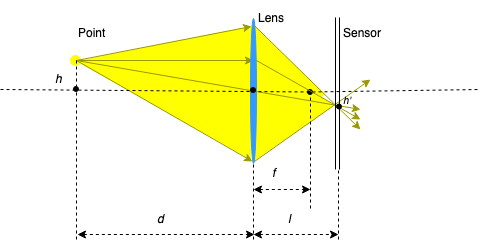
\includegraphics[width=0.9\textwidth]{../../images/lens.png}
 \caption{The refraction of rays through a thin focusing lens. Rays emitted by a point on the distance $d$ from the lens meet at a single point, which is at a distance $l$ from the lens.}
 \label{fig:lens}
\end{figure}

From Figure \ref{fig:lens} it is easy to derive the {\it lens formula}:

\begin{equation}
 \frac{1}{l} + \frac{1}{d} = \frac{1}{f}.
 \label{lens}
\end{equation}

This formula implies that if we place our sensor at distance the $l$ determined from \eqref{lens}, all the points which are at the same distance $d$ from the lens will be nicely projected on the sensor. Adjusting the position of the sensor to the lens will enable us to take sharp pictures of objects at different distances. 

The relations between the distances from the principal axis read:
\begin{equation}
h' = l\frac{h}{d}\equiv \frac{fh}{d-f}
\end{equation} 


{\bf What happens to the points which are at a slightly different distance?} or, equivalently,  {\bf What happens if we place the sensor in a slightly different location ?}

\begin{figure}[h]
\centering
 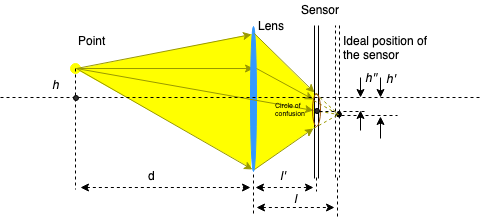
\includegraphics[width=0.9\textwidth]{../../images/lens_confusion_circle.png}
 \caption{The distorted image of the point caused by incorrect placement of the sensor. Note, the center of the circle of confusion is at a slightly different distance from the principal axis than the image of the point.}
 \label{fig:lens_cconf}
\end{figure}

Figure \ref{fig:lens_cconf} illustrates the process. The light cone focusing in the image of the point will be cut and, instead of a point we will have an illuminated disk - the {\it circle of confusion}. The photos taken by such a wrongly placed sensor will be blurred or {\it not in focus}. 

The distance between the center of the circle of confusion and the principle axis will be different from that of the point's image:
\begin{equation}
h'' = h'\frac{l'}{l} \equiv \frac{hl'}{d},
\label{dcirc}
\end{equation} 
where $h''$ is the distance between the center of the circle of confusion and the principal axis, $l$ is the ideal distance between the sensor and the lens, $h$ is the distance between the point and the principal axis and $h'$ is the distance between the image of the point on the ideally located sensor and the principal axis. See Figure \ref{fig:lens_cconf} .


It is clear from the diagram that depending on the diameter of the lens, the slight errors in the placement of the sensor can lead to a significant circle of confusion and, hence, blurring. Besides, the real world objects are not flat and we want to be able to make sharp photos of acceptable  sizes. We can control  the radius of the lens by placing a black screen with a small aperture right next to the lens (see Figure \ref{fig:lens_aperture}) 

\begin{figure}[h]
\centering
 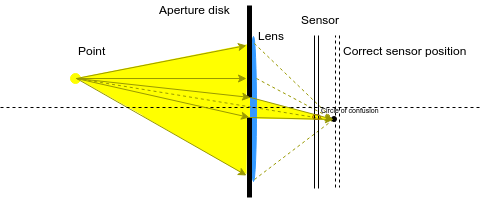
\includegraphics[width=0.9\textwidth]{../../images/lens_confusion_circle_aperture.png}
 \caption{The aperture disc reduces the circle of confusion }
 \label{fig:lens_aperture}
\end{figure}

Assuming that the sensor is placed at distance $l'\neq l$ from the lens, where $l$ is the correct distance determined from \eqref{lens} and that the diameter of the aperture is $D$, it is easy to derive the diameter of the circle of confusion $c$:
\begin{equation}
c = D\left(1-\frac{l'}{l}\right),
\end{equation} 
or, if we substitute the value of $l$:
\begin{equation}
c=D\left(1 -l' \left(\frac{1}{f} - \frac{1}{d}\right )\right )
\label{conf_circ_expanded}
\end{equation} 

Surprisingly,  the diameter does not depend on the distance of the point from the principle axis rather depends only on the distance of the point from the lens( $l$ depends on the d).  

Note, that placing the {\it aperture disk} between the object and the lens does not change the position of the image of the point. The ideally located sensor will feel the presence of the aperture disk only by the reduction of the reaching light amount. 

By sufficiently reducing the aperture diameter we can make the circle of confusion of any point smaller than the half of the sensor's pixel. Further reduction will not contribute to the sharpness (because we have reached the sensor's sharpness limit) but will rather  make the image only dimmer.

Obviously, the smaller the aperture diameter the deeper objects we can have in focus. 

Note, since the rays passing through the lens' center do not refract, in the limit of infinitely small aperture the presence of the lens can be neglected and this will turn into the pinhole camera described above. 

\subsection{Fixed focus cameras}

Since in the future posts we will mostly play with web cameras and the majority of webcams are so-called fixed-focus cameras, let us dive a little deeper into this particular corner case.

First of all, let us rewrite the formula \eqref{lens} as follows:
\begin{equation}
l=\frac{df}{d-f}\equiv\frac{f}{1 - f/d}.\label{ldist}
\end{equation}

Notice, that for sufficiently far objects $d >> f$ the denominator in \eqref{ldist} goes to one and, therefore, the ideal location of the sensor will be close to the focus. The typical focal length of the modern cameras bounces around $1-10 mm$ so this condition is satisfied with high precision for our everyday objects and distances ($\sim 1m$). We can assume that with high precision that the sensors of the fixed-focus webcams are placed in the focus of the lens. 

Now, if we substitute $l'=f$ in \eqref{conf_circ_expanded} two first terms will cancel each other and we will arrive to the following formula:

\begin{equation}
c=\frac{Df}{d}
\end{equation}

It is clear from the formula that the larger is $d$ the smaller is the circle of confusion $c$. So, for the fixed focal length $f$ and aperture diameter $D$ all points which are farther than $d_0$ from the lens
\begin{equation}
d_0 = \frac{Df}{c} \label{hyperfocal}
\end{equation}
will have a circle of confusion less than $c$. This is called {\it hyperfocal distance}. If for $c$ we take half the  size of our sensing pixel, all objects which are farther than \eqref{hyperfocal} from the lens will be as sharp as our sensor can possibly make. 

Finally, the distance of the image of the point from the principal axis, according to \eqref{dcirc} will read:
\begin{equation}
h'' = \frac{hf}{d}
\end{equation}

Comparing this to \eqref{pinhole_ratio} shows that we can use formulae  \eqref{projinhmg} for the fixed focus cameras.


\end{document}
